\chapter{General Introduction} \label{sec:intro}
\section{Background} %\section{Motivation}
%(Charbonneau et al. 2000; Henry et al. 2000), 
\paragraph{Transit technique}
The field of exoplanets has been evolving at an unprecedented rate: over 4000 planets have been discovered and many more candidates await confirmation (e.g., Coughlin et al. 2016; Morton et al. 2016). 
%-------exoplanet detection techniques
%Transit technique
%Transit Photometry
Most of the known planets were discovered with indirect methods such as the transit technique using NASA's Kepler space telescope (Borucki et al. 2010; see also Fig.~\ref{fig:stat}). The transit technique works by measuring the periodic dimming of the host star due to an orbiting planet. Since the dimming of the star is proportional to the size of the planet, it allows the planet’s radius to be measured if the host star's radius is also known. This technique is sensitive to large planets in short-periods, e.g. hot Jupiter (\cite{Mayor1995}), due to the higher probability of a transit occurrence in such configuration.  

%Transiting exoplanets are interesting objects to study because the coupling of radial velocity and photometric measurements allows a determination of stellar and planetary parameters and thus gives us an important constraint on fundamental models of planet formation and evolution. 
%From the light curve obtained during transit events, it is possible to measure the inclination of the orbit with respect to the line of sight and the size of the system’s components. Combining these results with spectroscopic measurements, we can obtain a precise value of the mass of the planet (rather than just a lower limit as for extrasolar planets detected by radial velocity measurements; Marcy & Butler 1998).

%Anomalies in the light curves of planetary transits can arise from several phenomena affecting the parent stars, such as grav- ity darkening (Barnes 2009; Szabó et al. 2011), stellar pulsation (CollierCameron et al. 2010), starspots (e.g. Sanchis-Ojeda et al. 2011; Tregloan-Reed et al. 2013) and even the presence of exo- moons (Kipping et al. 2009). 
%Hot Jupiters are gas-giant exoplanets with sizes like that of Jupiter but much shorter orbital periods. WASP-19b is the shortest-period hot Jupiter to be discovered so far, and has an excessively bloated radius, owing to the extreme radiation that it receives from its host star; as a result of this radiation, the planets effective temperature is more than 2,000 K (obtained via secondary eclipse measurements10)
%Tsiaras et al. 2017 presented a population study of 30 hot Jupiters (600K <T<2400 K and 0.35R$_{Jup}$<$R_p$<1.9 R$_{Jup}$ transmission spectra. 
\begin{figure}
\centering
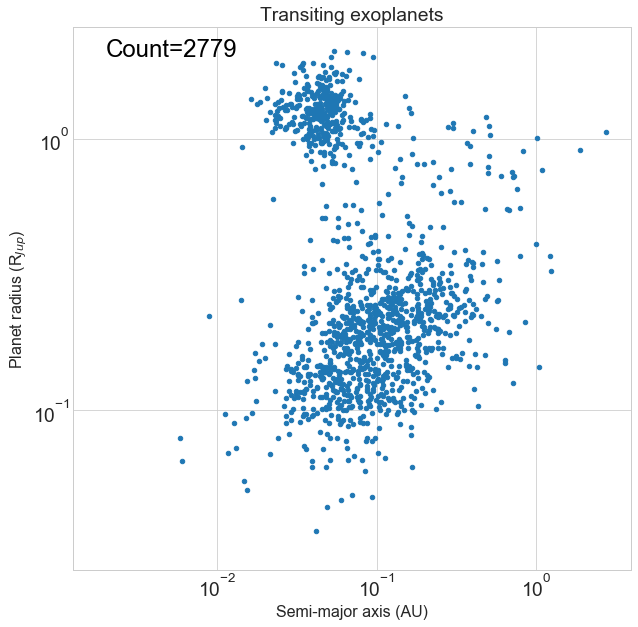
\includegraphics[width=7cm]{figures/statistics_a_vs_R.png}
\caption{Transiting exoplanets discovered to date. The diagram shows two general transiting planet populations based on radius and semi-major axis (i.e. hot Jupiter and mini Neptune). The data comes from NASA Exoplanet Archive retrieved on January 2018.}
\label{fig:stat}
\end{figure}

\paragraph{Bulk composition}
Moreover, if the planet’s mass is also known, %either via spectroscopic and radial velocity measurements, 
then combining mass with the radius determined via the transit technique yields the planet’s density which is the first step towards distinguishing between gaseous and rocky planets. 
%RV technique: 
%Radial Velocity Measurement
%The radius of the planet are directly imprinted on the transit lightcurve. Similarly, the radial velocity (RV) technique which measures the line-of-sight wobble of star due to the orbiting planet is sensitive to massive planets in short orbits around bright stars. The RV technique however provides mass information which together with radius derived from transit technique, yields the planet’s bulk density which is the first step towards distinguishing between gaseous and rocky planets. 
%Direct Imaging
%In comparison, direct detection method such as high contrast imaging which spatially resolves the planet from the star is sensitive to big, young and hence self-luminous sub-stellar objects and/or objects located far from their star such that their faint signal can be distinguished from the glare of the host star. 
Figure~\ref{fig:density} shows more than 500 exoplanets with measured mass and radius and the curves represent different (theoretical) planet  compositions ranging from pure light elements (e.g. H \& He) to dense metals (e.g. Iron). This plot demonstrates the compositional diversity that cannot be understood by studying the Solar System planets alone. Thus, studying exoplanets offers the perfect laboratory to test theories of planet formation. While density can help distinguish between gaseous and rocky exoplanets, it cannot provide information about the presence of trace elements, as well as its chemistry and dynamics. Thus, current research is focused towards detection and characterization exoplanet atmosphere because it offers the most reliable way to detect biosignatures and hence assess the planet's habitability (e.g., Burrows et al. 2014). 
\begin{figure}
\centering
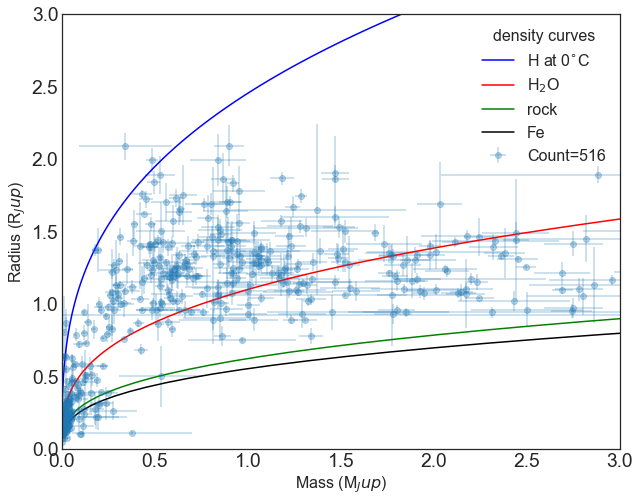
\includegraphics[width=7cm]{figures/density.png}
\caption{Compositional diversity of transiting exoplanets. More than 500 transiting exoplanets have measured mass and radius which provide constraint on their bulk density. Taking uncertainty into account, known exoplanets span a range of compositions from pure light elements (e.g. Hydrogen) to dense metals (e.g. Iron).}
\label{fig:density}
\end{figure}

%ground-based observation plays a vital role in validating and for further detailed characterization
%Although the interest in shifting towards M dwarfs
%ground-based telescope is still confined with relatively large gaseous planets 
%especially in the case of robustly detecting broad atmospheric signatures such as Rayleigh scattering with photometry
%hot Jupiters remain prime targets to accomplish this task
%Fukui+2016 demonstrated that MuSCAT can detect such atmospheric feature but for planets not currently available   
%Until the advent of TESS era and assuming its predicted discoveries come into fruition, we continue to improve transit modeling and more robust statistical modeling  
%Thus, the main targets of this thesis are hot Jupiters
%low density hot Jupiters offers the best chance to detect

%Fig.~\ref{fig:density} shows the mass-radius diagram of small exoplanets illustrating the diversity of their composition. The sparsity of objects in the diagram shows that terrestrial planets in the HZ are only beginning to present themselves. Similarly, the diagram shows the technical difficulties in obtaining reliable mass and radius measurements for solid exoplanets. The key to overcome this difficulty is to observe planets around late type stars. M-dwarfs for example have been shown to comprise 70\% of stars in the solar neighborhood (i.e. within 10 pc; Bochanski et al., 2010). Due to its proximity and frequency coupled with their smaller masses and radii, M dwarf systems hold the key to finding terrestrial planets in the habitable zone (HZ)—regions around the star where liquid water may exist and possibly life (Hart, 1979; Kasting et al., 1993). Indeed, most M dwarfs are now known to host closely-packed planetary systems characterized by a paucity of Jupiter-mass planets and the presence of multiple rocky planets, with roughly a third of these rocky M-dwarf planets orbiting within the HZ, including the three of the seven TRAPPIST-1 planets recently discovered (Gillon et al. 2017). Thus, M dwarfs have become prime targets for finding and characterizing terrestrial exoplanets. 
%The difficulty lies on the few known M dwarfs to date. 

%By now, more than 300 planets transiting their host star have been found, and much effort is being put into measuring the properties of each system. 

%\section{Transits and Occultations}
%When transiting in front of its host star, a planet blocks a fraction of the incident stellar light. The amount of blocked light relative to the original stellar light is called the transit depth. Since a set of transit depths observed at different wavelengths (called transmission spectrum) depends on atmospheric constituents, one can infer the atmospheric composition via multi-wavelength transit observations.

%\subsection{Transmission spectrum from transit observation}
%As a planet transits its parent star, some of the stellar flux passes tangentially through the planet's limb and upper atmosphere. For an extended atmosphere, the transit depth is wavelength-dependent. 

\paragraph{Exoplanet atmosphere}
During a transit, a small fraction of the starlight (e.g. 1–2\% for a typical hot Jupiter) %this can be confirmed in exoplanet plot pl_trandep
is blocked by the planet's opaque disk. On top of the disk, however, there is an optically-thin annulus (i.e. the exoplanet's upper atmosphere if present) through which incident light can be transmitted, absorbed, or scattered depending on the atmospheric properties. %Because the atmospheric opacity varies with wavelength, the apparent radius at which the planet's atmosphere becomes optically thick changes with wavelength (Seager \& Sasselov 2000; Brown et al. 2001; Hubbard et al. 2001). 

\begin{figure}
\centering
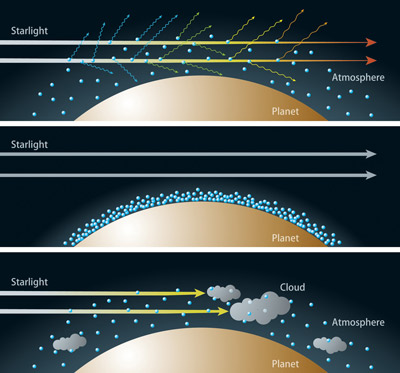
\includegraphics[width=7cm]{figures/atmosphere.jpg}
\caption{A cartoon illustrating the relationship between the composition of the atmosphere and transmitted colors of light. (credit: NAOJ)}
\label{fig:atm}
\end{figure}

If the sky has a clear, upward-extended, hydrogen-dominated atmosphere, Rayleigh scattering disperses a large portion of the blue light from the atmosphere of the host while it scatters less of the red light. As a result, a transit in blue light becomes deeper than the one in red light (see Fig.\ref{fig:atm} (top)). If the sky has a less extended, water-rich atmosphere, the effect of the Rayleigh scattering is much weaker than in a hydrogen-dominated atmosphere. In this case, transits in all colors have almost the same transit depths (see Fig.\ref{fig:atm} (b)). If the sky has aerosol\footnote{aerosol is loosely defined here as particles suspended in a gas and can refer to clouds, haze, and dust interchangeably}, most of the light cannot be transmitted through the atmosphere, even though hydrogen dominates it. As a result, transits in all colors have almost the same transit depths (see Fig.\ref{fig:atm} (c)). 

%\section{Rayleigh Scattering}
%\subsection{Theory}
%If the sky has a clear, upward-extended, hydrogen-dominated atmosphere, Rayleigh scattering disperses a large portion of the blue light from the atmosphere of the host while it scatters less of the red light. As a result, a transit in blue light becomes deeper than the one in red light.
%The transmission spectrum of a transiting planet therefore contains information about the scattering and absorption properties of the upper atmosphere near the planet’s day-night terminator.
In practice, this wavelength-dependent radius variation can be measured by multi-color photometry in which change in flux arising from rays that pass through the planet's atmosphere:
\begin{equation} 
\delta F_{\rm{transit}} = \frac{\pi(R^2-R^2_0)}{\pi R^2_s} \approx \frac{2R_0\delta R}{R^2_s}
\end{equation}
$\delta F_{\rm{transit}}$ is essentially an annulus of the atmosphere ($2\pi R_0 \delta R$), divided by the area of the stellar disk ($\pi R^2_s$). Here, the apparent radius $R=R_0+\delta R$ where $\delta R$ is the (small) deviation from the planet radius $R_0$ measured at some reference wavelength. The change in transit radius is usually some multiple of the (isothermal) scale height $H$: $\Delta R = nH$, with typical $n\sim 5$ depending on the spectral resolution and wavelength. 
The scale height, the vertical distance over which the gas pressure drops by a factor of $e$, is expressed as
\begin{equation} 
\label{eq:H}
H=\frac{kT_{eq}}{\mu g}
\end{equation}
where $k$ is the Boltzmann constant, $T_{eq}$ is the atmospheric temperature, $\mu$ is the mean molecular weight, and $g_p$ is the planetary surface gravity. Measuring $\delta F_{\rm{transit}}$ across several wavelengths constitutes the planet's transmission spectrum. 
%The mixing ratios of the absorbers and surface/cloud-top pressure, together with $\mu$ and $r_p$, are the atmospheric properties that affect (and can be inferred from) the spectrum.

%Several observations have been conducted to take the spectrum of exoplanets. Some spectra show 

\begin{comment}
\begin{figure}
\centering
\includegraphics[width=7cm]{figures/mancini.png}
\caption{Optical transmission spectrum of a hot Jupiter WASP-98 b where different models for clear (green), cloudy (yellow), hazy (blue), and best-fit (red) model are superposed to the measured optical spectrum (black data points) of the planet (Mancini et al. 2016)}
\label{fig:mancini}
\end{figure}
\end{comment}

%Additionally, multiple-band photometry of a TEP system can be used to constrain the composition of an exoplanet’s atmosphere. 
%sample sizes for is still too small to enable robust statistical investigations.
%Despite a great deal of theoretical work, the mechanism(s) by which hot Jupiters are emplaced onto misaligned orbits–and even whether an alternate mechanism, rather than tides, might actually be responsible for the trends described above–remains unclear.
%A variety of further observations are needed to distinguish among these models.

Although multi-color photometry generally does not have the power to resolve specific atoms or molecules, it is still useful to observe broad spectral features and test for the presence or absence of aerosol (e.g., Croll et al. 2011; de Mooji et al. 2012, 2013; Fukui et al. 2013, 2014; Mancini et al. 2013, 2014; Narita et al. 2013a,b; Nascimbeni et al. 2013, 2015).  

\paragraph{Aerosols in exoplanet atmosphere}
Presence of aerosol in the form of clouds and/or hazes in the exoplanet's atmosphere can be inferred based on the Rayleigh scattering signature detected in the optical wavelengths. %Any significant deviation from a flat line could mean anything between clear or cloudy atmosphere. 
Fig.~\ref{fig:atm_haze} shows a comparison of the transmission spectrum models with and without haze in the the atmosphere of a typical hot Jupiter. Between 0.5--5 $\mu$m, haze in the upper atmosphere %($P\lesssim 10^{-4}$ bar) 
causes radiation to become optically thick and prevent the molecules in the lower atmosphere %($P\gtrsim {10}^{-4}$ bar) 
such as H$_2$O, CH$_4$, and HCN from showing their absorption features. %Horizontal dotted lines represent the transit depths corresponding to the pressure levels from $1\times 10^{-6}$ bar to 1 bar for the atmosphere without haze. 
In the optical (0.3–1 $\mu$m), the spectral slope due to Rayleigh scattering by small ($\lesssim$ 0.1 $\mu$m) haze particles in the upper atmosphere can be seen. Thus, a relatively featureless spectrum in the near infrared and a large Rayleigh scattering in the optical can be used to infer the existence of haze in the atmosphere. 

\begin{figure}
\centering
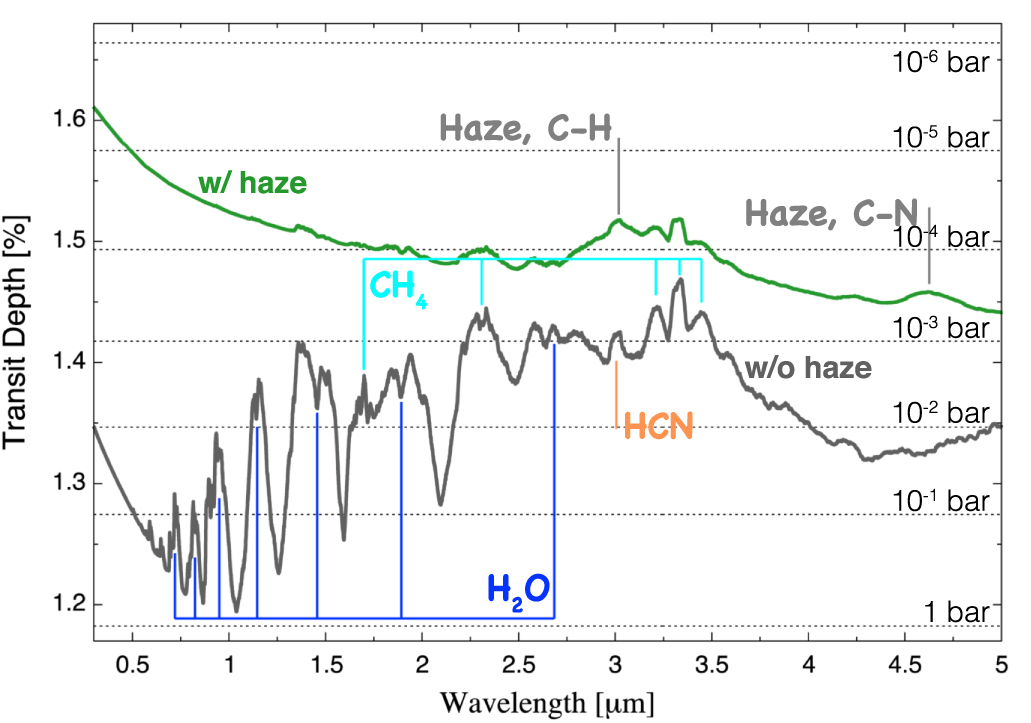
\includegraphics[width=8cm]{figures/haze_kawashima2017.jpg}
\caption{Transmission spectrum models for a clear atmosphere (black line) and  a hazy atmosphere (green line). Haze in the planet's upper atmosphere causes radiation to become optically thick and prevent the molecules in the lower atmosphere from showing their absorption features. A relatively featureless spectrum in the near infrared and a large Rayleigh scattering in the optical can be used to infer the existence of haze in the atmosphere. (credit: Fig.~9 in \cite{Kawashima2017})}
\label{fig:atm_haze}
\end{figure}



\begin{comment}
\subsection{Summary of Observation of Low Density Hot Jupiters}
%Investigation of atmospheric composition of transiting exoplanets by multi-band photometric observations with the aim of detecting variation of the planet’s radius as a function of wavelength has been conducted by a few groups recently (Southworth et al. 2012b; Mancini et al. 2013a,b,c;Nikolov et al. 2013).

So far, transit spectroscopy of exoplanets has been mainly performed on two hot Jupiters: HD209458b and HD189733b. Located at relatively close distances (47 and 19 pc, respectively), the two stars (G0V and K1-K2, respectively) have a visible magnitude V of 7.7, much brighter than the host stars of the other transiting hot Jupiters. 


%==========================================================================
\section{Observations of Low Density Hot Jupiters}
%hot Jupiters, including WASP-6b (Jordán et al. 2013; Nikolov et al. 2015) and WASP-31b (Sing et al. 2015). 

%An increase in planetary radius with decreasing wavelength in the atmosphere of the hot Jupiter HD 189733b is first reported by Pont et al. (2008) and Sing et al. (2011), based on Hubble Space Telescope (HST) Advanced Camera for Surveys and Space Telescope Imaging Spectrograph (STIS) observations, respectively. Pont et al. (2008) and Sing et al. (2011) demonstrate the effect is planetary rather than stellar, and they attribute it to the presence of Rayleigh scattering due to high-altitude hazes. 

%A few groups (Pont et al. 2008; Sing et al. 2011, 2015; de Mooij et al. 2013; Narita et al. 2013; Dragomir et al. 2015) conducted a search for the Rayleigh-scattering slope at optical wavelengths for smaller planets around.

%Narita et al. (2013) and de Mooij et al. (2013) have carried out such observations for GJ 1214b, a warm super- Earth orbiting a M dwarf, but found the transmission spectrum to be as featureless at these short wavelengths as it is at longer wavelengths (Berta et al. 2012; Fraine et al. 2013). 

%Notable examples are 55 Cnc e (Demory et al. 2011; Winn et al. 2011; V=5.95) and HD 97658b (Dragomir et al. 2013; V=7.7).  GJ 1214b (Charbonneau et al. 2009; V=14.7), GJ 436b (Gillon et al. 2007; V=10.6), and GJ 3470b (Bonfils et al. 2012; V=12.3), all of which orbit M dwarf (so smaller) stars, are such systems. This small, but growing, sample of favorable super-Earths, sub-Neptunes, and hot Neptunes continues to be the target of considerable effort to probe these planets' atmospheres via transmission spectroscopy (Seager \& Sasselov 2000; Brown 2001).

%So far, these observations often reveal featureless transmission spectra, which are interpreted as a high-mean-molecular-weight atmosphere and/or high-altitude hazes (Miller-Ricci et al. 2009; Kreidberg et al. 2014).

%These studies emphasize the importance of adequately characterizing the stellar variability and the spot properties when undertaking such analyses. 

%Fukui et al. (2016) demonstrated the ability of MuSCAT to probe atmospheric features of exoplanets larger than super-Earths (Fig. 5). Because known cool planets are too faint for ground-based telescopes, there are not enough targets to date observed with MuSCAT with sufficient precision.

%The first discovered exoplanet around a main sequence star is a hot Jupiter named 51 Peg b (\cite{Mayor1995}) thanks to its large radius and short period. 
%scale height
%Rayleigh scattering

%==========================================================================

Hot Jupiters—Jupiter-sized planets that orbit very close to the star, currently dominate spectral data of exoplanet atmospheres. A comparative study of ten hot Jupiter atmospheres reported a continuum from clear to cloudy atmospheres (Sing et al. 2016) wherein more irradiated atmospheres tend to have less clouds (Fig. 3; Heng et al. 2016). 

WASP-31b 
WASP-12b 
HAT-P-12b 
HD189733b 
WASP-6b

However, it is not known whether smaller, cooler planets follow the same trend. Although it is known that hydrocarbon haze particles can be produced via photochemical processes in low-temperature (T<1000 K) atmospheres such as that of Neptune and Uranus, empirical data is lacking to support this claim mainly due to the very few currently-known transiting low-temperature planets that are observable either on the ground or in space. However, this situation will be dramatically changed by TESS, which will detect hundreds of super-Earths/Neptunes around nearby M dwarfs (see Fig. 2). This offers MuSCAT2 a golden opportunity to follow-up new targets as soon as they become observable from the ground. Aside from confirming the new TESS candidates and refining their transit parameters, MuSCAT2 will be able to provide optical spectra in four bands that are generally useful to constrain the presence/absence and perhaps even degree of cloudiness of these cool or warm transiting exoplanets around nearby M dwarfs.


to obtain and constrain fundamental system parameters:
%==========================================================================
\end{comment}

\section{Motivation}\label{sec:followup}
%\section{Planet validation}
%follow-up observation/ validation/ detailed characterization
To confirm and characterize detected transiting systems, follow-up observations are necessary. %(see also $\S$\ref{sec:followup}). 
Generally, there are three methods for follow-up studies: (1) multi-color transit photometry used to measure any wavelength-dependent radius variation; (2) AO/lucky imaging to resolve any contaminating background stellar-mass sources; and (3) reconnaissance spectroscopy and RV measurements to measure mass limits of the companion. In this study, we focus on multi-color transit photometry. %Among the three planet validation methods, only multi-color transit photometry yields constraints on atmospheric properties of the planet. 

%Narita+2013
%Experiences have shown that broadband single-color transit photometry is not efficient to constrain an atmosphere model in the presence of starspots and the stellar variability. More effective ways to characterize atmospheres of transiting planets would be (1) simultaneous multi-color transit photometry using small-medium ground-based telescopes (e.g., Croll et al. 2011; de Mooij et al. 2012; Narita et al. 2013; Fukui et al. 2013b)

Multi-color transit photometry can eliminate false positive detections by measuring the change in the observed planet radius as a function of wavelength during the transit. For example, eclipsing binary stars, which can mimic the signal of a transiting planet, produce significant wavelength-dependent radius variation caused by stellar photosphere whereas a true planet produces weaker variation due to stellar limb darkening and its atmosphere if present. 
%One such survey is the multi-color Transiting (MuSCAT) project (Narita et al. 2014) which has been carrying out follow-up observations for 3 years now.
%Discovery of transiting exoplanet systems are mostly conducted by dedicated surveys (e.g. HAT-net). Follow-up observations are important to confirm the planetary nature of the transit signal and improve the properties of the system.
%Follow-up transit photometry can also improve the transit ephemeris which is useful for precise transit prediction in future observations. Checking for transit-timing variations (TTV) in several epochs can provide constraints on the existence and possibly mass of non-transiting companion(s) in the system. 
Precise measurement of transit depths (i.e. planet radius) at multiple wavelengths %(called transmission spectrum) 
provide independent constraint on atmospheric property. With an estimated planetary temperature and gravity, the detection of a Rayleigh scattering slope yields the atmospheric scale height which can then be used to estimate the mean molecular mass for general atmospheres independently of other atmospheric properties (\cite{Benneke2012}). 
%The wavelength dependence of transit depth can also be used to characterize the atmospheres. In particular, the linear slope of the Rayleigh scattering signature %or the shapes of individual features
%provide constraints on the atmosphere scale height 
%first detection of atmosphere (Charbonneau 2002)
Moreover, detection of Rayleigh scattering slope in the optical usually by ground-based facilities is complementary to near-infrared transmission spectrum obtained usually using space telescopes. For example, GJ 3470b has been found to exhibit a flat transmission in the infrared which is interpreted as either due to a clear atmosphere with high-mean-molecular-weight or high-altitude  hazes (\cite{Kriedberg2014}; See also Fig.~\ref{fig:atm_haze}). Detection of Rayleigh scattering in the optical by \cite{Dragomir2015} help break such degeneracy by favoring an atmosphere model with hydrogen/helium-dominated atmosphere covered by hazes which obscure absorption features in the IR and hazes which give rise to scattering in the visible. This demonstrates the possibility to characterize the atmospheres of exoplanets using shorter-wavelength measurements even when their IR transmission spectra are featureless.
%We find that the most plausible scenario is a hydrogen/helium-dominated atmosphere covered by clouds which obscure absorption features in the infrared and hazes which give rise to scattering in the visible.

Most detections of Rayleigh scattering have been found in giant exoplanets with low densities since Rayleigh scattering signal is larger for planets with larger scale heights (See Eq.~\ref{eq:H}). Small planets transiting somewhat fainter stars are also accessible to existing facilities if their transits are deeper than the order of 0.1\% for a system with a smaller host star and/or a larger planet. Despite the large numbers of known or candidate planets, and despite the ubiquity of planets around small late-type stars, the host stars of most systems known to date are too faint for the detection and characterization of exoplanet atmospheres especially using ground-based telescopes.
This problem is compounded by the fact that light curves of planetary transits often contain deviations from a simple transit shape, and it is generally difficult to differentiate between anomalies of astrophysical nature (e.g. starspots) and correlated noise due to instrumental or atmospheric effects.

%While it is important to enlarge the number of detected planets, it is also vital to accurately measure the main physical properties of each planetary system used in statistical analysis.

Recent observations of transiting hot Jupiters using the Space Telescope Imaging Spectrograph (STIS) and Wide Field Camera 3 (WFC3) on the Hubble Space Telescope (HST) have revealed a variety of atmospheric characteristics. Most notably, the 10 hot Jupiters reported in Sing et al. (2016) 
%(for additional details of observations, see Huitson et al. 2013; Line et al. 2013a; Mandell et al. 2013; Pont et al. 2013; Sing et al. 2013, 2015; Wakeford et al. 2013; McCullough et al. 2014; Nikolov et al. 2014, 2015) 
indicate a variety of atmospheres, interpreted as a continuum of clear to hazy conditions. The diversity of these results emphasizes the need to increase the current pool of studied gas giant atmospheres to better understand the physical properties of low density hot Jupiters and the parameters governing the presence or absence of hazes. 

%Although it is known that hydrocarbon haze particles can be produced via photochemical processes in low-temperature (T<1000 K) atmospheres such as that of Neptune and Uranus, empirical data is lacking to support this claim mainly due to the very few currently-known transiting low-temperature planets that are observable either on the ground or in space. However, this situation will be dramatically changed by TESS, which will detect hundreds of super-Earths/Neptunes around nearby M dwarfs (see Fig. 2). This offers MuSCAT2 a golden opportunity to follow-up new targets as soon as they become observable from the ground. Aside from confirming the new TESS candidates and refining their transit parameters, MuSCAT2 will be able to provide optical spectra in four bands that are generally useful to constrain the presence/absence and perhaps even degree of cloudiness of these cool or warm transiting exoplanets around nearby M dwarfs.

%Thus, factors motivate additional observations in this wavelength regime.
Motivated by this need, we carry out simultaneous, multi-color transit photometry of low-density hot Jupiters with the goal of refining the physical parameters of such systems and searching for broad atmospheric features using a dedicated instrument discussed in the next section.

\section{OAO/MuSCAT\label{sec:muscat}}
%%%%%%%%%%%%%%%%%%%%%%%%%%%%MuSCAT%%%%%%%%%%%%%%%%%%%%%%%%%%%%%%%%%%%
%We report a development of a multi-color simultaneous camera for the 188-cm telescope at Okayama Astrophysical Observatory in Japan. The instrument, named MuSCAT (multi-color Simultaneous Camera for studying Atmospheres of Transiting exoplanets), has a capability of three-color simultaneous imaging in optical wavelengths where CCDs are sensitive. MuSCAT is equipped with three 1024 × 1024 pixel CCDs which can be controlled independently. The three CCDs detect lights in g2′ (400 to 550 nm), r2′ (550 to 700 nm), and zs,2 (820 to 920 nm) bands using Astrodon Photometrics Generation 2 Sloan filters. The field of view of MuSCAT is 6.1×6.1  arc min2 with the pixel scale of 0.358  arc sec/pixel. The principal purpose of MuSCAT is to perform high-precision multi-color transit photometry. For this purpose, MuSCAT has the capability of self-autoguiding which enables it to fix the positions of stellar images within ∼1 pixel. We demonstrate relative photometric precisions of 0.101%, 0.074%, and 0.076% in g2′, r2′, and zs,2 bands, respectively, for GJ 436 (magnitudes in g′=11.81, r′=10.08, and z′=8.66) with 30-s exposures.

For this study, we used the multi-color Simultaneous Camera for studying Atmospheres of Transiting exoplanets (MuSCAT), which is an optical three-band instrument that was recently developed for the 188 cm telescope at the Okayama Astrophysical Observatory (OAO; \cite{Narita2015a}). 
MuSCAT has three three CCD cameras equipped with the Sloan $g'_2$, $r'_2$, and $z_{s,2}$ filters (hereafter g-, r-, z-bands), which can obtain images in three bands simultaneously (\cite{Narita2015a}). Each CCD has pixel scale of 1".5 pixel$^{-1}$ and FOV of 5.6' $\times$ 5.6' . Technical specifications are summarized in Table~\ref{tab:muscat}.
MuSCAT has demonstrated its capability to achieve precision photometry with nominal error of rms(5-min)~0.02 for Vmag=10 star as in the case of HAT-P-14b (\cite{{Fukui}2016a}).
MuSCAT has also been successful in confirming and characterizing transiting exoplanets ranging from hot Neptunes (e.g., \cite{Narita2017}) to super-Earths in the habitable-zone (\cite{Fukui2016b}). 

\begin{table}
\centering
\caption{OAO/MuSCAT basic specification.} \label{tab:muscat}
\begin{tabular}{lll} \hline
             &Value      \\ 
\hline
Primary mirror & 1.88 m \\
Location       & 34$^{\circ}$34'37"N 133$^{\circ}$35'38" E, 372m \\
Filters  \multirow{3}{*}{} & g'$_2$: 400-550nm \\
                           & r'$_2$: 550-700nm \\
                           & z$_{s,2}$: 820-920nm \\
FOV    & 6.1'x 6.1' \\
Pixel scale & 0.36'' / pix \\ 
\hline
\end{tabular}
\end{table}

\begin{figure}
\centering
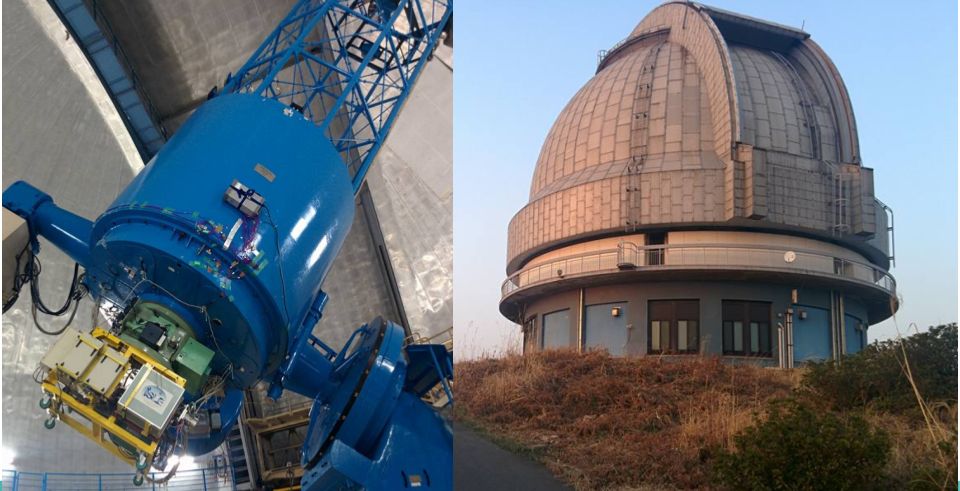
\includegraphics[width=7cm]{figures/oao-muscat.png}
\caption{OAO/MuSCAT}
\label{fig:muscat}
\end{figure}

%detecting a tiny (0.06%) transit of the K2 habitable-zone super-Earth K2-3d (Fukui et al. 2016b). It has also been used for validating transiting planetary candidates discovered from K2, as a part of the ESPRINT/KESPRINT collaboration (Hirano et al. 2016a, Narita et al. 2017).

%Moreover, Cabrera et al. (2017) demonstrated the importance of independent confirmation of planetary candidates after demoting the statuses of previously the validated planets K2-78b, K2-82b, and K2-92b into eclipsing binaries. % https://arxiv.org/pdf/1707.08007.pdf

%==========================================================================
\section{Targets: Hot Jupiters}\label{sec:targets}
We consider three targets for this thesis: HAT-P-44, HAT-P-12, and WASP-21 which were observed as part of on-going follow-up observation of transiting exoplanets with MuSCAT. 
%The main reason for selecting this system for a pilot observation is that a good comparison star with a similar brightness to the host star (V=9.6) exists within the FOV (HIP 84832; separated from HAT-P-14 by 4 4), offering a good opportunity to achieve a high photometric precision. Stars
These targets are chosen based on the planets' relatively low mean densities and hence large scale heights which therefore increases their likelihood to have a gaseous atmosphere on top of a solid surface. The expected scale height is computed using Eq. \ref{eq:H} assuming $\mu$=2.3 for H-H2 dominated atmospheres. %strongly irradiated and inflated giant planets
The stars' and planets' properties are summarized in Table~\ref{tab:params} and the observation log is summarized in Table~\ref{tab:obs}. Unless a more reliable measurement is available, the values are taken from discovery papers: HAT-P-44: \cite{Hartmann2014}; HAT-P-12: \cite{Hartmann2009}; WASP-21: \cite{Bouchy2010}. We summarize each system as follows.

%Short summary of our targets
%HAT-P-12: http://exoplanet.eu/catalog/HAT-P-12_b/
%ApJ, 834:50 (15pp), 2017 January 1
\paragraph{HAT-P-12b}
%HAT-P-14b (aka WASP-27b), a hot Jupiter orbiting a bright (V=10.1) F-type star in a retrograde and slightly eccentric (e= 0.1) orbit with the period of 4.63 days (Torres et al. 2010; Simpson et al. 2011; Winn et al. 2011). So far only one photometric follow up observation has been reported after the discoveries (Nascimbeni et al. 2011), leaving room for further photometric follow-ups to search for such as TTVs, TDVs, and transit- depth variations.
HAT-P-12b was detected with the HAT-5 telescope of the Hungarian-made Automated Telescope Network %(Bakos et al. 2004) 
in 2006. \cite{Hartmann2009} %Hartman et al. (2009) 
conducted follow-up photometry of four transits together with
spectroscopic observations and reported that the planet has a mass smaller than Saturn's and radius similar to Jupiter's, respectively, in a 3.2 day circular orbit around a fairly bright (m$_V$=12.8) K4-type star. 
%Its host star is a K4 dwarf (V = 12.8) with MA = 0.73 ± 0.02 M, RA = 0.70+0.02 −0.01 R.
%Since HAT-P-12b is one of the lowest-density planets orbiting metal-poor host stars, the physical properties of the system are important for irradiation models.
%HAT-P-12 b is also a low-surface gravity ($g_p$=5.6 ms$^-2$) % 0.295 ± 0.025 g cm–3
%\cite{Lee2012} reported three more follow-up transit observations to improve the properties of the system  using empirical calibrations from eclipsing binary stars and stellar evolutionary models. 
HAT-P-12b has many interesting properties. \cite{Hartmann2009} noted its unusually large scale height (615.6 km) which is at least an order of magnitude larger than Saturn's. It is also one of the lowest-density ($\sim$0.32 g cm$^{-3}$) planets with a fairly warm temperature $T_{eq}$=963 K %for a hot Jupiter  
orbiting metal-poor host stars. Due to these reasons, HAT-P-12b has been the subject of extensive follow-up observations both from ground and space (e.g. \cite{Lee2012}; \cite{Todorov2013}; \cite{Sing2016}). %and atmospheric modeling using its spectrum (e.g. \cite{Todorov2013}; \cite{Line2013}; \cite{Stevenson2016}). %high albedo >0.8 accdg to Barstow+17

%A LOW-DENSITY SUB-SATURN MASS PLANET TRANSITING A METAL-POOR K DWARF
In particular, HAT-P-12b reported \cite{Line2013} its transmission spectrum obtained using the Hubble Space Telescope's (HST) WFC3 instrument which showed lack of water absorption feature expected for a hydrogen-dominated atmosphere, favoring a model with high-altitude clouds. Subsequent observations using HST/STIS in the optical and Spitzer/IRAC in the infrared by \cite{Sing2016} reported it to be one of the 10 hot Jupiter samples with strong optical scattering slopes. More recently, \cite{Barstow2017} confirmed that HAT-P-12b's transmission spectrum is consistent with the presence of Rayleigh scattering due to atmospheric aerosol/ haze. 

Given a wealth of information, HAT-P-12b is included in our sample as a test case for verifying the results of our transit analysis.
%extending to low atmospheric pressures (below 0.1 mbar).
% In general, planets with equilibrium temperatures between 1300 and 1700 K are best represented by deeper, gray cloud layers, whereas cooler or hotter planets are better fit using high Rayleigh scattering aerosol. 
%In concordance with previous studies, we find that vertically homogeneous, small particle (<0.1 µm) clouds are best at producing strong Rayleigh scattering signatures, but only if iron-bearing cloud species are neglected. (Molliere+2017)

\paragraph{HAT-44}
%For HAT-P-44 we find that the preferred model, based on the estimated Bayes Factor, consists of two planets, the outer one on an eccentric orbit. This model includes: the transiting planet HAT-P-44b with a period of P = 4.301219 ± 0.000019 days, a mass of M p = 0.352 ± 0.029 M J , and an eccentricity of e = 0.044 ± 0.052; an outer planet HAT-P-44c with a period of P = 872.2 ± 1.7 days, a minimum mass of M p sin i = 4.0 +1.4 −0.8 M J , and an eccentricity of e = 0.494 ± 0.081. We adopt the model with the long period and high eccentricity for the outer component because it has the highest Bayes factor.
%\cite{Hartmann2014} report the discovery of HAT-P-44b identified using the HATNet telescopes, and then confirmed through follow-up observations with a variety of ground-based facilities. 
HAT-P-44b was detected with the HAT-5 telescope of the Hungarian-made Automated Telescope Network %(Bakos et al. 2004) 
in 2006. \cite{Hartmann2014} %Hartman et al. (2009) 
conducted follow-up photometry of five transits from 2010-2011 together with two spectroscopic observations and reported that the planet has a mass and radius % M=0.35,  R=1.24 
both slightly larger than Saturn and Jupiter, respectively, in a slightly eccentric (e=0.04) %0.044±0.052) 
4.3-day orbit around a relatively faint (m$_V$=13.2) G-type star.
%mass of 0.35 $M_J$, and radius of 1.24 R$_J$ yielding a density of 0.23 $\pm$ 0.04 (\cite{Hartmann2014}). 
Similar to HAT-P-12b, HAT-P-44b is a bloated planet with similar density of $\sim$0.23 g cm$^{-3}$ (\cite{Hartmann2014}) with a large scale height of $\sim$ 708 km.

Follow-up RV observation reveal significant systematic variations in its residual radial velocities, indicating the presence of an outer non-transiting companion. Combined RV+transit modeling indicate that HAT-P-44 consists of two planets, including the transiting component, with the outer planet having a period of 872 days, eccentricity of 0.494 $\pm$ 0.081, and a minimum mass of 4.0 M$_J$.
%In this regard, it is important to check whether transit timing variation can be detected from out photometric observation. (PERIOD TOO LONG!)

So far only few photometric follow up observations have been reported for HAT-P-44b which are included in the discovery paper (\cite{Hartmann2014}), leaving room for further photometric follow-ups to search for possible transit-timing variation (TTV), transit duration variation (TDV), and transit-radius variation (TRV). The follow-up photometric observations of HAT-P-44b was previously conducted using $r$ and $i$-bands but only a single Rp/Rs measurement are reported. Hence, this study will report the first ever search for such variations.

%The preferred model has an associated jitter of 10.7 ± 2.0 m s −1 and a χ 2 per degree of freedom, including this jitter, of 1.67. Based on Equation (1), one expects only 1.2\% of stars like HAT-P-44 to have jitter values 10.7 m s −1 thus the excess scatter in the RV residuals from the best-fit two-planet model suggests that perhaps more than two planets are present in this system, though we cannot conclusively detect any additional planets from the data currently available.

\paragraph{WASP-21}
%https://exoplanetarchive.ipac.caltech.edu/cgi-bin/DisplayOverview/nph-DisplayOverview?objname=WASP-21+b&type=CONFIRMED_PLANET
WASP-21b was detected with the SuperWASP-North telescope
in 2006. \cite{Bouchy2010} %Hartman et al. (2009) 
conducted follow-up photometry of five transits in 2008 together with eight spectroscopic observations and reported that the planet has a mass and radius % M=0.35,  R=1.24 
similar to Saturn and Jupiter, respectively, in a circular 4.3-day circular orbit around a relatively bright (m$_V$=11.6) G-type star.

%Bouchy et al. (2010) discovered this planetary system, and obtained its physical properties using their version of the dEB constraint. They obtained adaptive-optics imaging which show no faint stars contaminating the flux from the system. The interest in WASP-21 lies in its Saturn-mass planet (Mb = 0.295 ± 0.030MJup) and the metallicity which is the lowest known for a TEP host star (? Fe H ? = −0.46±0.11). Barros et al. (2011) analysed LT/RISE observations covering three transits, of which the firstwas originally presented in the discovery paper (Bouchyet al. 2010).They used theY2 models to provide their additional constraint, yielding significant differences compared to those found by Bouchy et al. (2010): MA = 0.86 ± 0.04M?versus 1.01±0.03M?,andMb=0.27±0.01M?versus 0.300±0.011M?.WASP-21

Similar to HAT-P-12b, WASP-21b is a bloated planet with similar density of $\sim$0.32 g cm$^{-3}$ (\cite{Bouchy2010}) around a metal-poor host. 

\cite{Barros2011} and \cite{Ciceri2013} found lower values for the mass and the density of the planet (by 1.0 and 1.4$\sigma$ respectively) with respect to those found in the discovery paper. In either case, the planet has a scale height of $\sim$ 900 km, the largest among our sample.%, and also reported no indication of TTV. 
%However, in a later study Barros et al. (2011a) found the G3V star to be in the process of moving off the main sequence. Thus, we included further observations of WASP21b planetary transits to improve the knowledge on this system.
%photometric follow-up and stellar density modeling from transit light curve by Barros 2011 report a stellar mass of 0.86 ± 0.04 M⊙, which is significantly lower than previously reported (1.01 ± 0.03 M⊙). Consequently, we find a lower planetary mass of 0.27 ± 0.01 MJup. 
As in the previous analyses, \cite{Barros2011}, \cite{Ciceri2013}, \cite{Seelinger2015} found no trend or sinusoidal variation in the system parameters.

WASP-21b was previously conducted using $r$ and $i$-bands but only a single Rp/Rs measurement are reported. Hence, this study will report the first ever search for such variations.

\begin{comment}
%Sensitivity to atmospheric feature
\paragraph{Achievable Measurement Error of Rp/Rs with MuSCAT}
%chapter 4.3 in 
\cite{Fukui2016a} simulated the achievable measurement error of Rp/Rs with MuSCAT. Three types of planet were considered: (1) the V = 10 F-dwarf HAT-P-14, (2) the nearby (38 pc) K-dwarf HAT-P-11 (Bakos et al. 2010), and (3) the nearby (14 pc) M-dwarf GJ1214 (Charbonneau et al. 2009). 

When a planet has an atmosphere with no thick clouds, $R_p/R_s$ can vary with wavelength by up to several $\times H/R_s$.
Therefore, if $\sigma_{Rp/Rs}$ is comparable to or smaller than the expected value of $H/R_s$, then it can roughly be considered that the measurement is sensitive to the atmosphere.
 
Given $T_{eq}$ and $g_p$ and assuming $\mu$=2.3, we can use Eq.~\ref{eq:H} to estimate the expected atmospheric scale height of our targets. 
Then, we can compute for the expected %$\sigma_{Rp/Rs}$ 
rms by assuming that the achievable precision for our targets will ideally follow the Poisson distribution. In the best case, the highest photometric precision achieved using MuSCAT is typically $\sim$0.028\% for HAT-P-14 with 5-minute binning (Vmag=10; \cite{Fukui2016a}). Since 
\begin{align*}
m_1-m_2 &= -2.5\log_{10}(f_1/f_2)\\
\rightarrow \frac{f_1}{f_2} &= 10^{\Big(\frac{m_2-m_1}{2.5}\Big)}\\
%\frac{f_1}{f_2} &= 10^{\Big(\frac{13.2-10}{2.5}\Big)} = 19.9
%\frac{f_1}{f_2} &= 10^{\Big(\frac{12.8-10}{2.5}\Big)} = 13.1
%\frac{f_1}{f_2} &= 10^{\Big(\frac{11.6-10}{2.5}\Big)} = 4.36
\end{align*}
%The photometric noise/ uncertainty goes with . Thus, the increase in the expected noise should be
and Poisson noise decreases by a factor $f=\sqrt{f_1/f_2}$ for our fainter targets, then $f$=4.47, 3.63, and 2.08 and hence $\sigma_{Rp/Rs}$=0.125, 0.101, 0.058 for HAT-P-44 (Vmag=13.1), HAT-P-12 (Vmag=12.8), and WASP-21 (Vmag=11.6), respectively. %The residual rms for g-band with 5 minute binning is 0.23\%, compared to Fukui-san's 0.028\%; an order of magnitude difference. We have to reduce the rms of the residual by a factor of 5 to match the photometric precisison expected for a Vmag=13 star.


% The right vertical axis of Figure 6 shows a scale in the unit of the expected scale height, assuming an isothermal atmosphere with the equilibrium temperature of $T_{eq}$=1624 K (Southworth 2012) and a solar abundance with $\mu$ = 2.35g. The 1$\sigma$ uncertainties of the measured Rp/Rs is the level of ∼10–20 times as large as one scale height.
\end{comment}

\begin{table}
\centering
\caption{Stellar and planetary parameters of our targets.}
\label{tab:params}
\begin{tabular}{lllll} \hline
          &HAT-P-44      &HAT-P-12        &WASP-21   \\ \hline
$R_s (R_{\odot})$     &0.949$^{+0.08}_{-0.037}$&0.701$^{+0.017}_{-0.012}$ & 1.060 $\pm$ 0.04 \\
$M_s (M_{\odot})$    &0.942$\pm$0.041   &0.730 $\pm$ 0.018 &1.010 $\pm$ 0.03 \\ 
SpT  & K & K4  & G3V \\
$V_{mag}$ &13.2              &12.8            &11.6               \\
age (Gyr) &7.5$\pm$3.6       &2.5$\pm$2.0     &12$\pm$5           \\ \hline
 &HAT-P-44b      &HAT-P-12b        &WASP-21b    \\ \hline
P (d) & 4.301219 $\pm$ 0.000019  & 3.21306 $\pm$ 0.000002    &  4.322482 $\pm$ 0.000024 \\
$R_p (R_{\rm{Jup}})$&      1.242$\pm$0.106  & 0.959$\pm$0.029& 1.07$\pm$0.06 \\
$M_p  (M_{\rm{Jup}})$ &   0.352$\pm$0.029   & 0.211$\pm$0.012 & 0.300$\pm$0.011 \\
$\bar \rho$  (g cm$^{-3}$) &  0.23$\pm$0.04   &0.3192$\pm$0.0160   & 0.32$\pm$0.07    \\ % 0.295 ± 0.025 Hartmann+09
$g$  (m$s^{-2}$) & 5.62$\pm$0.01   & 5.62$\pm$0.01 & 5.07$\pm$0.035 \\ 
%logg (cgs) 2.75 ± 0.03 Hartmann+09 
$T_{eq}$  (K) & 1108$^{+51}_{-32}$   & 963$\pm$16   & 1340$\pm$32  \\
$H$ (km) & 708.2 & 615.6 & 950.0 \\
\hline
\end{tabular}
\end{table}

\section{Contents}
In this thesis, new observations for low density hot Jupiters including HAT-P-12b, HAT-P-44b, and WASP-21b in search for TTV, TDV, and TRV are reported. % and their atmosphere models. 
The rest of the paper is organized as follows. Chapter $\S$ \ref{sec:obs} summarize the observations and methods of data reduction. Chapter $\S$ \ref{sec:results} describes the analyses of new transit light curves %and stellar variability. 
$\S$ \ref{sec:discussion} presents the results of the above analyses and discusses the implications. Finally, this thesis is summarized Chapter in $\S$ \ref{sec:summary}.